
%%%%%%%%%%%%%%%%%%%%%%% file typeinst.tex %%%%%%%%%%%%%%%%%%%%%%%%%
%
% This is the LaTeX source for the instructions to authors using
% the LaTeX document class 'llncs.cls' for contributions to
% the Lecture Notes in Computer Sciences series.
% http://www.springer.com/lncs       Springer Heidelberg 2006/05/04available
%
% It may be used as a template for your own input - copy it
% to a new file with a new name and use it as the basisfig
% for your article.
%
% NB: the document class 'llncs' has its own and detailed documentation, see
% ftp://ftp.springer.de/data/pubftp/pub/tex/latex/llncs/latex2e/llncsdoc.pdf
%
%%%%%%%%%%%%%%%%%%%%%%%%%%%%%%%%%%%%%%%%%%%%%%%%%%%%%%%%%%%%%%%%%%%


\documentclass[runningheads,a4paper]{llncs}
\usepackage[utf8]{inputenc}
\usepackage{amssymb}
\setcounter{tocdepth}{3}
\usepackage{graphicx}

\usepackage{url}
%\urldef{\mailsa}\path|{jmoura, andrea}@inf.ufsm.com.br|    
\newcommand{\keywords}[1]{\par\addvspace\baselineskip
\noindent\keywordname\enspace\ignorespaces#1}

\begin{document}

\mainmatter  % start of an individual contribution

% first the title is needed
\title{
Test automation on BPMS applications: \\ An Experience with two Open Source BPM Systems}

% a short form should be given in case it is too long for the running head
\titlerunning{
Test automation BPMS applications: \\ an Experience Report}

% the name(s) of the author(s) follow(s) next
%
% NB: Chinese authors should write their first names(s) in front of
% their surnames. This ensures that the names appear correctly in
% the running heads and the author index.
%
\author{Jéssica Lasch de Moura
%\thanks{Please note that the LNCS Editorial assumes that all authors have used
%the western naming convention, with given names preceding surnames. This determines
%the structure of the names in the running heads and the author index.}%
\and Andrea Schwertner Charão}
%
\authorrunning{
Test automation of BPMS applications: \\ an Experience Report}
% (feature abused for this document to repeat the title also on left hand pages)

% the affiliations are given next; don't give your e-mail address
% unless you accept that it will be published
\institute{Computer Science Nucleus\\
Universidade Federal de Santa Maria -- UFSM\\}
%\mailsa
%\mailsb\\
%\mailsc\\
%\url{http://www.springer.com/lncs}}

%
% NB: a more complex sample for affiliations and the mapping to the
% corresponding authors can be found in the file "llncs.dem"
% (search for the string "\mainmatter" where a contribution starts).
% "llncs.dem" accompanies the document class "llncs.cls".
%

\toctitle{Lecture Notes in Computer Science}
\tocauthor{Authors' Instructions}
\maketitle


\begin{abstract}
%The abstract should summarize the contents of the paper and should contain at least 70 and at most 150 words. It should be written using the \emph{abstract} environment.
This article describes an experience of test automation of an application developed with the support of Business Process Management Systems - BPMS. For this purpose, we have implemented the same process using different versios of two different BPMS: Bonita and Activiti. We submit the resulting Web applications to two types of tests (load tests and functional tests), using test tools Selenium, Cucumber, Apache JMeter and TestNG. The results show the feasibility and limitations of test automation for this type of application.

%\keywords{We would like to encourage you to list your keywords within the abstract section}
\end{abstract}


\section{Introduction}

%A gestão de processos de negócio (\emph{Business Process Management} -- BPM) tem suscitado o interesse de empresas e da comunidade científica, tanto por seus benefícios como por seus desafios. Designa-se por BPM o conjunto de conceitos, métodos e técnicas para suportar a modelagem, administração, configuração e análise de processos de negócio~\cite{weske}. Associados a isso, surgiram os sistemas BPM (\emph{Business Process Management Systems} -- BPMS), que são ferramentas de software para apoio ao ciclo de vida da gestão de processos de negócio. 

Business Process Management has aroused the interest of companies and the scientific community, both for their benefits as per their challenges. Is called of BPM a set of concepts, methods and techniques to support the modeling, administration, configuration and analysis of business processes  ~\cite{weske}. Associated with this, emerged the BPM systems (\emph{Business Process Management Systems} -- BPMS), which are software tools to support the life cycle of business process management.

%Dentre os diversos BPMS disponíveis atualmente, é comum encontrar ferramentas com suporte à modelagem, configuração e execução de processos de negócio. Em muitos casos, os BPMS abreviam o desenvolvimento de software, entregando aplicações Web completas para execução dos processos, usando tecnologias atuais e exigindo pouca escrita de código. Por outro lado, algumas tarefas como verificação e testes ainda são consideradas um desafio nesta área~\cite{aalst2013survey}. Em particular, o teste automatizado de aplicações de BPMS é pouco abordado, tanto pela comunidade da área de BPM~\cite{weske} como da área de testes de software~\cite{graham2012experiences}. 

Among the many BPMS currently available, it is common to find tools that support modeling, configuration and execution of business processes. In many cases, BPMS shorten the software development, delivering complete Web applications for process execution, using current technologies and requiring little code writing. On the other hand, some tasks such as checking and tests are still considered a challenge in this area ~\cite{aalst2013survey}. In particular, the automated test of BPMS applications is rarely addressed by both the BPM community ~\cite{weske} as software testing area~\cite{graham2012experiences}.
 
%No entanto, a falta de automação nos testes pode levar a problemas durante a implementação e execução de processos de negócio, ainda mais quando se tratam de processos com muitas tarefas e fluxos de trabalho, que levam facilmente a explosões combinatórias.
However, the lack of automation in testing can lead to problems during implementation and execution of business processes, especially when treating processes with many tasks and workflows, which easily lead to combinatorial explosion.

%O propósito deste trabalho foi explorar soluções para teste automatizado de um processo implementado em BPMS. Para isso, partiu-se de uma aplicação real, em que testes manuais se revelaram insuficientes~\cite{sbsi2013}. No presente artigo, relata-se a experiência com testes automáticos nesta aplicação, utilizando-se ferramentas \emph{open source}. A aplicação é apresentada na seção \ref{s:apli}, após uma discussão sobre BPM e testes na seção \ref{s:bpmtest}. Na sequência, a seção \ref{s:testes} apresenta os métodos, ferramentas e resultados obtidos em cada tipo de teste. Por fim, a seção \ref{s:conclu} resume as lições aprendidas.

The purpose of this study was to explore solutions for automated testing of a process implemented in BPMS. For this, it started with a real application where manual testing proved inadequate~\cite{sbsi2013}. In this article, we report the experience with automated testing this application, using open source tools. The application is presented in section \ref{s:apli}, after a discussion of BPM and tests in section \ref{s:bpmtest}. Further , the section \ref{s:testes} presents the methods, tools and results of each type of test. Finally, the section \ref{s:conclu} summarizes the lessons learned.
%deixar citaçoes ao trabalho em protugues?


\section{BPM and Testing}\label{s:bpmtest}

%O termo BPM pode ser usado com ênfases diferentes, às vezes com foco em tecnologia (software) e outras vezes em gestão. Mesmo assim, a área tem convergido no entendimento do ciclo de vida de aplicações de BPM, que envolve as atividades de análise, modelagem, execução, monitoramento e otimização~\cite{ABPMP}. Também há convergência sobre o padrão BPMN (\emph{Business Process Model and Notation}) para expressar a modelagem de processos.

The BPM term can be used with different emphases, sometimes focusing on technology (software) and other times management. Still, the area has converged in understanding the lifecycle of BPM applications, involving the analysis of activities, modeling, execution, monitoring and optimization~\cite{ABPMP}. There is also convergence on the pattern BPMN (\emph{Business Process Model and Notation}) to express the process modeling. 
%citaçao em portugues?

%Os sistemas de BPM (BPMS) têm se afirmado como ferramentas essenciais para suporte a atividades desse ciclo de vida. Atualmente, pode-se dizer que um típico BPMS oferece recursos para definição e modelagem de processos em BPMN, controle da execução e monitoramento de atividades dos processos~\cite{forrester}. Há uma tendência dos BPMS em abreviar o desenvolvimento de software, por exemplo através de geradores de formulários Web associados a tarefas dos processos~\cite{greenresearch}. Nota-se, no entanto, que a preocupação com testes não fica evidente nas ferramentas BPMS. De fato, examinando-se o material promocional e a documentação disponível sobre os principais BPMS, observa-se uma ênfase em etapas de modelagem e execução.

BPM systems (BPMS) has been claimed as essential tools to support the activities of this life cycle. Currently, it can be said that a typical BPMS provides resources for definition and process modeling in BPMN, execution control and activity monitoring of processes~\cite{forrester}. There is a tendency of BPMS in shortening software development, for example via web forms generators associated with process tasks~\cite{greenresearch}. Note, however, that the concern with testing is not evident in the BPMS tools. Indeed, examining the promotional material and documentation available on the main BPMS, there is an emphasis on modeling and execution stages.


%Por outro lado, a importância dos testes é amplamente reconhecida em engenharia de software~\cite{swebok14}. 
%Considerando que aplicações de BPMS são geralmente sistemas baseados na Web, pode-se supor que sejam testadas com sucesso usando-se abordagens consagradas, como por exemplo testes de carga ou testes funcionais do tipo caixa-preta. Há também quem argumente que o teste de aplicações de BPM difira do teste de aplicações Web tradicionais~\cite{evoke}, porém não foram encontradas mais referências aprofundando esse ponto de vista. Essa constatação reforçou a motivação para o presente trabalho.
Moreover, the importance of the tests is widely recognized in software engineering ~\cite{swebok14}. 
Whereas BPMS applications are usually Web-based systems, it can be assumed that it can be successfully tested using dedicated approaches, such as load tests or functional testing of the black-box type. There are also those who argue that BPM applications test differs from traditional Web applications testing~\cite{evoke}, but there were no more references to deepen this view. This finding reinforced the motivation for this work. 


\section{Test Target Application}\label{s:apli}

%A aplicação alvo deste trabalho refere-se a um processo comum em instituições de ensino superior: a apreciação de Atividades Complementares de Graduação (ACGs), ou seja, atividades que formam a parte flexível do currículo de graduandos (participação em palestras, eventos, projetos, etc.). Em um trabalho anterior ~\cite{sbsi2013}, apresentou-se a modelagem, implementação e implantação desse processo. Sua representação em BPMN, na Figura \ref{fig:diagrama}, revela um total de 11 tarefas distribuídas em 5 divisões de responsabilidade (Aluno, Tutor, etc.).

The target application of this work refers to a common process in higher education institutions: the appreciation of complementary activities, ie, activities that form the flexible part of the undergraduate curriculum (participation in lectures, events, projects , etc.). In a previous work ~\cite{sbsi2013}, presented the modeling, implementation and deployment of this process. Their representation in BPMN, in Figure \ref{fig:diagrama}, reveals a total of 11 tasks span responsibility 5 divisions.
%citando trabalho em portugues

In that previous work, we implemented the process with the Bonita BPM tool \footnote{Bonita BPM (formerly Bonita Open Solution). Available at: www.bonitasoft.com} in version 5.7.2, an open source BPMS recognized in the corporate world ~\cite{forrester}. The resulting application has several Web forms for each division of responsibility, being the first one for the data population by the student. According to the type of complementary activities, the flow is directed to those responsible for the assessment and validation of activity. Note, in Figure \ref{fig:diagrama}, the process has several gateways, which leads to over 15 possible different paths in the process.

\begin{figure}[ht]
\centering
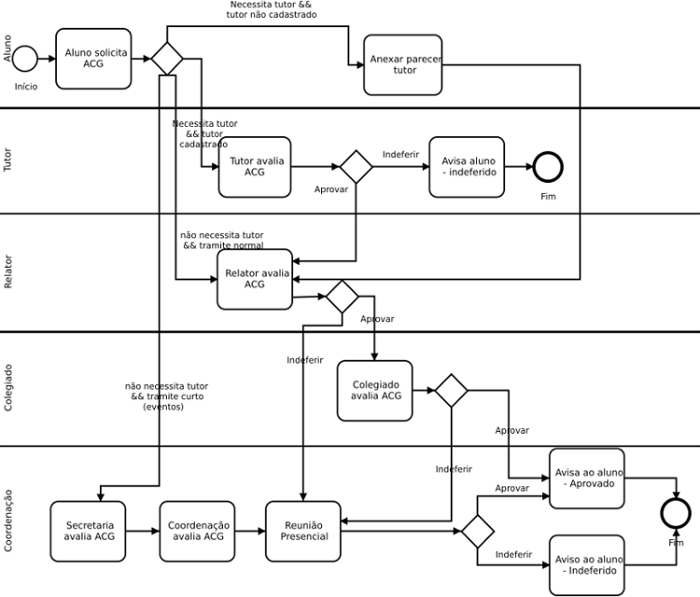
\includegraphics[width=0.9\textwidth]{figuras/processo.png}
\caption{BPMN process diagram}
\label{fig:diagrama}
\end{figure}

%A aplicação foi submetida a testes funcionais realizados manualmente, além de testes de aceitação realizados com um grupo de usuários reais. Entretanto, com algumas semanas em operação, surgiram problemas: instâncias do processo falharam devido a entradas inesperadas, serviços não foram restabelecidos corretamente após serem interrompidos e houve sobrecarga devido ao grande número de casos abertos numa data limite. Essa experiência motivou a busca de soluções para automação de testes.
The application was subjected to functional testing performed manually, in addition to acceptance testing with a group of real users. However, a few weeks in operation, problems emerge: Process instances failed due to unexpected inputs, services were not restored properly after being interrupted and there was overloaded because of the number of cases opened on a deadline. This experience led to the search for solutions for test automation.

%Verificou-se, no entanto, que o BPMS utilizado não possuía suporte a nenhum tipo de teste automatizado. Buscou-se outros BPMS com licenças \emph{open source} ou \emph{freeware}, que pudessem implementar o processo em questão e que oferecessem suporte a testes. A preferência por este tipo de licença foi devida à sua flexibilidade e viabilidade financeira para o ``cliente'' deste projeto: uma instituição pública de ensino.
It was found, however, that the BPMS used does not support any type of automated testing. We attempted to other BPMS with open source or freeware licenses, which could implement the process in question and offered testing support. The preference for this type of license was due to its flexibility and affordability to the "client" of this project: a public educational institution.

%Dentre as ferramentas analisadas (TIBCO\footnote{TIBCO. Disponível em: www.tibco.com.}, Activiti\footnote{Activiti. Disponível em: www.activiti.org.}, Process Maker\footnote{Process Maker. Disponível em: www.processmaker.com.}, Intalio\footnote{Intalio. Disponível em: www.intalio.com.}), nenhuma oferecia evidente suporte a testes automatizados. Apenas a ferramenta Activiti citava a possibilidade de testes de unidade aliados ao JUnit, porém sem muitas informações sobre essa alternativa. Por isso partiu-se para outra opção: utilizar ferramentas de teste externas ao BPMS. 
Among the analyzed tools (TIBCO\footnote{TIBCO. Available at: www.tibco.com}, Activiti\footnote{Activiti. Available at: www.activiti.org}, Process Maker\footnote{Process Maker. Available at: www.processmaker.com}, Intalio\footnote{Intalio. Available at: www.intalio.com}), none offered clear support for automated testing. Just Activiti tool cited the possibility of allies unit tests to JUnit, but are not cited much information about this alternative. So we went to another option: use test tools external to BPMS.

%Adicionalmente, decidiu-se implementar a mesma aplicação usando outro BPMS, a fim de ampliar a experiência e, possivelmente, identificar semelhanças e diferenças no teste automatizado de implementações com diferentes BPMS. Porém, não tinha-se como objetivo eleger o melhor BPMS, mas sim avaliar suporte aos testes considerados. 
In addition, it was decided to deploy the same application using other BPMS in order to broaden the experience and possibly identify similarities and differences in automated test implementations with different BPMS. Yet it had intended to elect the best BPMS, but to assess support for both tests.

%A ferramenta escolhida foi Activiti, um BPMS baseado em tecnologias Java, assim como Bonita, permitindo trabalhar com as mesmas tecnologias do lado servidor (Tomcat e MySQL, no caso em questão). Esse BPMS também trabalha com a mesma versão da notação BPMN usada no Bonita, permitindo importar na íntegra o processo originalmente criado. Os formulários Web criados com ajuda do Bonita, no entanto, não puderam ser importados e tiveram de ser recriados com Activiti.
%The tool chosen was Activiti, a BPMS based on Java technologies, like Bonita, allowing you to work with the same server-side technologies (Tomcat and MySQL, in this case). At the time, the latest version of the application was 5.14. This BPMS also works with the same version of the BPMN notation used in Bonita, allowing import in full the process originally created. Web forms created with Bonita's help, however, could not be imported and had to be recreated with Activiti. %escrever sobre as versoes diferentes aqui?
%Os testes foram realizados em dois momentos diferentes utilizando as versoes mais recentes de cada ferramenta. Assim, foram testadas aplicaçoes criadas com a versao 5.7.2 e 7.1.2 do Bonita e versao 5.14 e 5.19 do Activiti.
The tool chosen was Activiti, a BPMS based on Java technologies, like Bonita, allowing you to work with the same server-side technologies (Tomcat and MySQL, in this case). This BPMS also works with the same version of the BPMN notation used in Bonita, allowing import the full process originally created. Web forms created with Bonita's help, however, could not be imported and had to be recreated with Activiti. The tests were performed at two different times using the latest versions of each tool. Thus, were tested applications created with the 5.7.2 and 7.1.2 version of Bonita and version  5.14 and 5.19 of the Activiti. 

\section{Description and Execution of tests}\label{s:testes}

%No planejamento de testes automatizados, priorizou-se o teste de aspectos que de fato revelaram problemas durante a implantação, no trabalho precedente. Os testes escolhidos foram: (a) testes de carga, que são um tipo de teste de desempenho, visando avaliar o comportamento do sistema frente a um grande número de solicitações e (b) testes funcionais, a fim de verificar as saídas do sistema produzidas a partir de entradas pré-definidas. Nenhum destes tipos de teste possui suporte nos BPMS Bonita e Activiti, que incluem somente funcionalidades limitadas de simulação e depuração de execução dos processos. Embora o Activiti citasse suporte a testes de unidade, não explorou-se esta opção por entender-se que seria menos prioritária frente aos problemas observados.
In planning automated tests, priority was given to the test of aspects that in fact revealed problems during deployment in previous work. The selected tests were: (a) functional tests to verify the produced system output from pre-defined inputs and, (b) load tests, which are one type of performance testing, to evaluate the behavior of the system  opposite to a large number of requests. None of these types of tests is supported in BPMS Bonita and Activiti, which include only limited functionality simulation and debugging process execution. Although Activiti quoting support unit tests  this option will not be exploited for to be understood that would be less priority compared to the observed problems.

%Assim, realizou-se um levantamento de ferramentas destinadas ao teste de aplicações Web e selecionou-se as julgadas mais promissoras, antes de partir-se para o detalhamento e execução dos testes. Os \emph{scripts} que configuram os testes estão disponíveis para consulta em http://www.inf.ufsm.br/~andrea/bpmtest-scripts.zip.
Thus, there was a survey of tools intended for Web application testing and was selected the most promising judged before departing to the detailing and execution of tests. The scripts that configure the tests are available for consultation in http://www.inf.ufsm.br/$\sim$andrea/bpmtest-scripts.zip.

\subsection{Functional Tests}

%Para executar testes funcionais em aplicações Web, pode-se utilizar ferramentas livres como Selenium\footnote{Selenium. Available at: www.seleniumhq.org.}, Watir\footnote{Watir. Available at: www.watir.com.} ou Geb\footnote{Geb. Available at: www.gebish.org.}. Para este trabalho, escolheu-se a ferramenta Selenium, aliada ao Cucumber-JVM\footnote{Cucumber-JVM. Available at: www.github.com/cucumber/cucumber-jvm.} para descrição dos testes. A escolha foi motivada pelo grande número de referências ao Selenium na Web, confirmadas por um trabalho que apresentou resultados satisfatórios com Selenium e Cucumber~\cite{sbqs2013}.

To perform functional tests on Web applications, you can use free tools like Selenium\footnote{Selenium. Available at: www.seleniumhq.org.}, Watir\footnote{Watir. Available at: www.watir.com.} or Geb\footnote{Geb. Available at: www.gebish.org.}.For this work, we picked up the Selenium tool, combined with Cucumber-JVM \footnote{Cucumber-JVM. Available at: www.github.com/cucumber/cucumber-jvm.} for a description of the tests. %The choice was motivated by the large number of references to the Selenium web, confirmed by a work which showed satisfactory results with Selenium and Cucumber ~ \ cite {} sbqs2013.

%Com estas ferramentas, o processo para a execução de um teste funcional é composto de: captura da interação do usuário com o navegador (Selenium IDE), exportação do código gerado (Selenium IDE), criação do cenário de teste (Cucumber), criação das definições dos passos do teste (Cucumber), criação dos métodos para cada passo (Java) e execução do teste (Selenium WebDriver). O cenário de teste é a definição, em ordem de execução, dos passos que são executados na aplicação, bem como dos resultados esperados. Para este trabalho, definiu-se um cenário em que o aluno faz login e preenche 2 formulários referentes à primeira tarefa do processo e após isso um outro usuário faz o login e executa a segunda tarefa do processo disponibilizada para ele. Para este cenário, foram criados métodos variando as entradas nos formulários. Como o processo testado é o mesmo em todos os BPMS, o cenário de teste também é o mesmo. 

With these tools, the process for running a functional test consists of: capture the user interaction with the browser (Selenium IDE), export the generated code (Selenium IDE), creation of test scenario (Cucumber), creation of definitions of test steps (Cucumber), creation of methods for each step (Java) and test execution (Selenium WebDriver). The test scenario is a definition, in order of execution of steps that run the application, and the expected results. For this work, it was set up a scenario in which the student logs in the application and fills 2 forms as a first task of the process and after that another user logs in and runs the second task of the process available to him. For this scenario, methods were created by varying the entries on the forms. As the tested process is the same in all BPMS, the test scenario is also the same.
%For this work, was set up a scenario in which the student logs in and fills 2 forms as a first task of the process. For this scenario, methods were created by varying the entries on the forms. As the tested process is the same in both BPMS, the test scenario is also the same.
%adicionei mais uma etapa em todos os testes com as duas versões da ferramenta

%Para as aplicações de ambos os BPMS, inicialmente ocorreram erros na execução dos testes, relativos à localização de campos nos formulários Web. Verificou-se que os campos estavam localizados em um \emph{iframe} e, embora a captura da interação ocorresse sem problemas, o código gerado não selecionava o \emph{iframe} e por isso não encontrava os campos. Assim, foi necessário utilizar um método do Selenium para acessar o \emph{iframe} antes de selecionar o elemento desejado.


%Em um trabalho anterior, foram testadas as versões 5.7.2 do Bonita e 5.14 do Activiti. Nestes primeiros testes foi analisada a execução de apenas uma tarefa do processo e, devido a isso, foi utilizado um cenário diferente. Como forma de ampliar a experiência, foram então realizados testes também com as versões mais recentes dos BPMS sendo elas: 7.1.2 do Bonita e 5.19 do Activiti. Também foi atualizado o cenário de teste para as 4 versões diferentes, a fim de ser testada mais uma tarefa.%

In a previous work~\cite{sbqs2015}, versions 5.7.2 Bonita and 5.14 Activiti were tested. In these first tests was analysed only one task of the process, and because of this, were used a different scenario. As a way to broaden the experience also tests were then carried out with the latest versions of BPMS: 7.1.2 of Bonita and 5.19 of Activiti. Also the test scenario has been updated for the four different versions in order to be tested one more task. In the Figure \ref{fig:cenario2}, can be viewed the scenario used in the tests with the four versions.

\begin{figure}[ht]
\centering
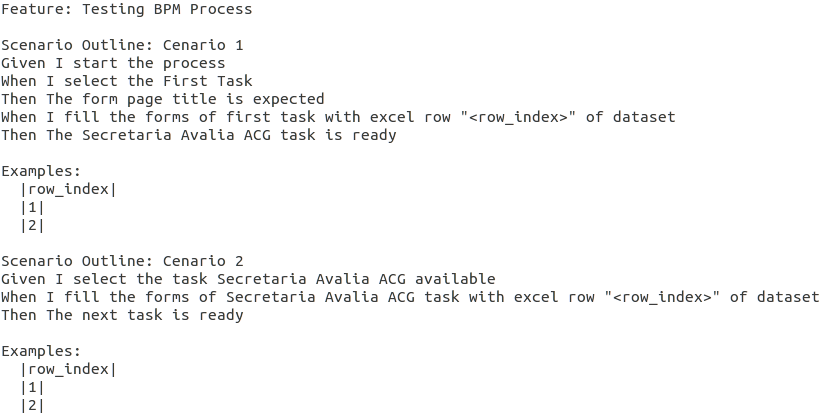
\includegraphics[width=0.9\textwidth]{figuras/cenario2.png}
\caption{Test Scenario}
\label{fig:cenario2}
\end{figure}


For applications created with both versions of each BPMS, initially errors occurred in the tests relating to the location of the fields in web forms. It was found that the fields were located in a \emph{iframe}, while the capture of the interaction to occur without problems, the generated code did not select the \emph{iframe} and so could not find the fields. Thus, it was necessary to use a Selenium method to access the \emph{iframe} before selecting the desired element.

%Na aplicação com Activiti, ocorreu também outro problema. Diferente do que ocorreu com os formulários Web gerados pelo Bonita, o Selenium IDE não capturou toda a interação do usuário com a aplicação. De fato, na etapa de login, o Selenium capturou apenas o acesso à página e o ``clique'' ao botão de login, ou seja, não capturou o preenchimento dos campos ``Usuário'' e ``Senha''. Este problema se repetiu com alguns outros elementos do formulário Web durante a gravação da interação. Acredita-se que o problema ocorra devido à estrutura das página Web, que pode conter elementos que o Selenium não identifique automaticamente, tais como \emph{divs}, \emph{frames} e \emph{scripts}, por exemplo. No entanto, isso não impossibilita a criação e execução dos testes. Para contornar o problema, foi necessário estudar a estrutura das páginas Web em questão, localizar os elementos faltantes e então adicionar o código para acessá-los nos respectivos métodos.
%Este problema não ocorreu com a versão 5.19 do Activiti assim como nas duas versões do Bonita, a captura e execução dos elementos ocorreu com sucesso sen do apenas necessárias algumas pequenas alterações no código gerado.

In application with version 5.14 of Activiti also ran into other trouble. Unlike what happened with the Web forms generated by Bonita, the Selenium IDE did not capture all user interaction with the application. Indeed, in the login stage, Selenium just captured the access page and the `` click '' to the login button, ie not captured filling the fields `` User '' and `` password ''. This problem was repeated with some other elements of the Web form when recording the interaction. It is believed that the problem occurs due to the structure of the Web page, which can contain elements that Selenium does not automatically identify, such as \emph{divs}, \emph{frame} and \emph{scripts}, for example. However, this does not preclude the creation and execution of tests. To work around the problem, it was necessary to study the structure of the Web pages in question, locate the missing elements and then add the code to access them in their methods. 

This problem did not occur with the version 5.19 of Activiti as well as in the two versions of Bonita, the capture and execution of the elements was successful it was only needed some minor changes in the generated code.

\subsubsection{Functional Tests Results}
%Os testes funcionais mostraram-se mais viáveis do que os testes de carga, pois uma boa parcela da interação é executada no lado cliente, sem necessidade de lidar explicitamente das interações com o servidor. Pode-se dizer que este teste atingiu todos seus objetivos, pois permitiu reproduzir a interação do usuário, bem como criar o código para testar as aplicações com diferentes entradas, num cenário envolvendo a tarefa inicial do processo, ampliando a cobertura dos testes. O  teste funcional também reproduziu erros encontrados em produção e que tinham passado despercebidos nos testes manuais (entradas não previstas corretamente nos formulários), esses erros foram os mesmos em ambas as ferramentas BPMS, pois os formulários foram configurados de modo equivalente. 
%The functional tests were more viable than load tests, because a good part of the interaction is performed on the client side without the need to explicitly handle the interactions with the server. It can be said that this test reached all its goals because it allowed reproduce user interaction and create the code to test applications with different inputs in a scenario involving the initial task of the process, expanding the coverage of the tests. Functional testing also reproduced errors found in production and that had gone unnoticed in manual tests (not properly provided for in the forms entries), these errors were the same in both BPMS tools because the forms were configured equivalently.
%Os testes funcionais mostraram-se viáveis, uma boa parcela da interação é executada no lado cliente, sem necessidade de lidar explicitamente das interações com o servidor. Pode-se dizer que este teste atingiu todos seus objetivos, pois permitiu reproduzir a interação do usuário, bem como criar o código para testar as aplicações com diferentes entradas, num cenário envolvendo duas tarefas iniciais do processo, ampliando a cobertura dos testes. O  teste funcional também reproduziu erros encontrados em produção e que tinham passado despercebidos nos testes manuais (entradas não previstas corretamente nos formulários), esses erros ocorreram nas duas versões de ambas as ferramentas BPMS, pois os formulários e entradas testados foram configurados de modo equivalente. 
The functional tests proved to be viable, mainly because a good portion of the interaction is performed on the client side without the need to explicitly handle the interactions with the server. It can be said that this test reached all its goals because it allowed reproduce user interaction and create the code to test applications with different inputs, in a scenario involving two initial tasks of the process, expanding the coverage of the tests. Functional testing also reproduced errors found in production and that had gone unnoticed in manual tests (not correctly expected inputs in forms), these errors occurred in the two versions of both BPMS tools because forms and tested entries were configured equivalently.

%O teste funcional também foi menos dependente do BPMS. Na Tabela \ref{tab:testeFuncional} apresenta-se um resumo das principais semelhanças e diferenças encontradas. Em ambos os casos, foram necessárias poucas modificações no código gerado pelo Selenium e Cucumber, bastando para isso inspecionar a estrutura das páginas Web. O Cucumber torna a implementação dos testes mais rápida e menos trabalhosa do que se fosse usado apenas o Selenium, abreviando a geração de código alinhado com os cenários de teste. Mesmo assim, caso seja necessário estender os testes a muitas tarefas de um processo, as modificações no código de teste podem se tornar trabalhosas.

%Functional testing was also less dependent on BPMN. The Table \ref{tab:testeFuncional} presents a summary of the main similarities and differences found. In both cases, it took a few modifications to the code generated by the Selenium and Cucumber simply by inspecting the structure of Web pages. Cucumber makes the implementation of testing faster and less labor than if it were used only Selenium, shortening the code generation aligned with the test scenarios. Still, if necessary to extend the test to many tasks of a process, changes in the test code may become laborious.
As it was possible to realize the tests successfully on all the tools and code testing is similar (only required a few modifications), it is possible to say that the functional test is little dependent to the chosen BPMS. Table \ref{tab:testeFuncional} presents a summary of the main similarities and differences found. In all cases, it took a few modifications to the code generated by the Selenium and Cucumber by simply inspecting the structure of web pages. Cucumber makes the implementation faster and less labor than if it were used only Selenium, shortening the code generation aligned with the test scenarios. Still, if necessary to extend the test to many tasks of a process, changes in the test code may become laborious.

%\begin{table}
%\centering
%\begin{center}
%{\scriptsize
%\begin{tabular}{p{6cm}|l|p{4.5cm}}
%\hline
% & Bonita & Activiti \\\hline
%Web Technologies & HTML, CSS, Ajax & HTML, CSS, Ajax \\\hline
%Capture of user interaction using Selenium & Total & Partial (required manual insertion of some fields) \\\hline
%It was possible to export the code generated by Selenium? & Yes & Yes \\\hline
%Recognition of all fields captured WITHOUT code change & Partial & Partial \\\hline
%Recognition of all fields captured WITH code change & Total & Total \\\hline
%\end{tabular}
%}
%\caption{Comparative overview of the functional test}
%\label{tab:testeFuncional}
%\end{center}
%\end{table}

\begin{table}
\centering
\begin{center}
%{\scriptsize
\begin{tabular}{p{3cm}|p{2cm}|p{2.5cm}|p{2.5cm}|p{2.5cm}}
\hline
 & Bonita 5.7.2 & Bonita 7.1.2 & Activiti 5.14 & Activiti 5.19 \\\hline
Web Technologies & HTML, CSS, Ajax & HTML, CSS, Ajax & HTML, CSS, Ajax & HTML, CSS, Ajax \\\hline
Capture of user interaction using Selenium & Total & Partial (required manual insertion of some fields) & Partial (required manual insertion of some fields) & Partial (required manual insertion of some fields) \\\hline
It was possible to export the code generated by Selenium? & Yes & Yes & Yes & Yes\\\hline
Recognition of all fields captured WITHOUT code change & Partial & Partial & Partial & Partial \\\hline
Recognition of all fields captured WITH code change & Total & Total & Total & Total \\\hline
\end{tabular}
%}
\caption{Comparative overview of the functional test}
\label{tab:testeFuncional}
\end{center}
\end{table}


\subsection{Load Tests}
%Os testes de carga inicialmente foram realizados utilizando a ferramenta JMeter\footnote{Apache JMeter. Available at: www.jmeter.apache.org} no entanto, devido a problemas encontrados durante a execuçao dos testes, tambem foi utiizada uma versao alterantiva de teste atraves do Selenium. Nos testes de carga foi avaliado o desempenho da execuçao da primeira tarefa da processo, pois esta pode ser considerada um "gargalo" devido ao grande numero de usuarios que pode iniciar um processo simultaneamente.

%Load tests were first conducted using the JMeter tool. However, due to problems encountered during the tests, it was also used an alternative test using Selenium. 
In the load testing it was evaluated the performance of the execution of the first task of the process as it can be considered a "bottleneck" because of the number of users who can start a process simultaneously.

%Testes de carga em aplicações Web são tipicamente realizados gerando-se múltiplas requisições HTTP ao servidor, de forma controlada. Para isso, uma etapa crítica é a identificação das requisições que devem ser reproduzidas. Existem diversas ferramentas que se propõem a facilitar este tipo de teste, dentre as quais pode-se citar: JMeter\footnote{Apache JMeter. Disponível em: www.jmeter.apache.org.}, The Grinder\footnote{The Grinder. Disponível em: www.grinder.sourceforge.net/.} e WebLOAD\footnote{WebLOAD. Disponível em: radview.com/webload-download/.}. Todas são ferramentas \emph{open source} e possuem diversas opções, mas escolheu-se a ferramenta JMeter pela sua funcionalidade ``proxy server'' que é de grande auxílio à captura das requisições.
\subsubsection{Load Tests with Apache JMeter}
Load tests on web applications are typically performed by generating multiple HTTP requests to the server in a controlled manner. For this, a critical step is to identify the requests that should be reproduced. There are several tools that purport to facilitate this type of testing, among which we can mention: JMeter, The Grinder\footnote{The Grinder. Available at: www.grinder.sourceforge.net/} and WebLOAD\footnote{WebLOAD. Available at: www.radview.com/webload-download/}. All tools are open source and have several options, but chose to JMeter tool for its functionality "proxy server" which is a great help to the capture of requests.

%Um teste da aplicação com JMeter consiste em quatro etapas: capturar as requisições HTTP, exportar as requisições (formato .jrxml para JMeter), configurar o plano de teste e, por fim, executar o teste no JMeter. A aplicação gera diferentes requisições HTTP que precisam ser identificadas e interpretadas, para serem reproduzidas automaticamente. O emprego de tecnologias Web com processamento assíncrono, do lado do cliente, pode dificultar esta etapa, pois uma ação do usuário pode não gerar imediatamente uma requisição ao servidor. Além disso, em aplicações de BPMS, diversos usuários atuam sobre diferentes tarefas de um mesmo processo, de modo que as requisições HTTP carregam chaves identificando usuários e processos.
An application test with JMeter consists of four steps: capture HTTP requests, export requests (.jrxml format for JMeter), set up the test plan and, finally, run the test in JMeter. The application generates different HTTP requests that need to be identified and interpreted to be played automatically. The use of Web technologies with asynchronous processing, client-side, can hinder this step because a user action can not immediately generate a request to the server. Moreover, in BPMS applications, many users act on different tasks in a same process, so that the HTTP requests that carry user identifying keys and processes.

%No caso da aplicação criada com Bonita, verificou-se que existe uma chave identificadora de sessão que é gerada no momento em que usuário acessa o sistema e outra chave identificadora de instância, ou seja, que identifica cada execução do processo como única, sendo criada pelo servidor no momento em que o usuário inicia o processo. Para executar os testes, portanto, foi necessário localizar a requisição em que essas chaves são geradas e utilizar a ferramenta ``Extrator de Expressão Regular'' do JMeter para obter seus valores. Já na aplicação criada com Activiti, foi inviável identificar a requisição em que as chaves são geradas, pois não há uma requisição cujo retorno (resposta do servidor) contenha valores de chaves. Esta situação leva a crer que a geração das chaves identificadoras é feita internamente pelo BPMS, ou seja, não em uma requisição HTTP e, por consequência, esta não pode ser capturada e reproduzida no JMeter.
In the case of application created with Bonita in the version 5.7.2, it was found that there is a session identifier key that is generated at the time user accesses the system and other instance identifying key, that is, identifies each execution of the process as only being created by the server when the user initiates the process. To run the tests, so it was necessary to locate the request in which these keys are generated and use the "Regular Expression Extractor" tool of JMeter to get their values. In the application created with Activiti in the version 5.14, it was impossible to identify the request in which the keys are generated, as there is not a request whose return (server response) contains key values. This suggests that the generation of the identifying key is made internally by the BPMS, ie not in an HTTP request and therefore this can not be captured and reproduced in JMeter.

% colocar uma nova seçao aqui? 
%Novos testes de carga com selenium + TestNG
%Para expandir a experiencia, decidiu-se realizar o teste de carga com as versões atualmente mais recentes das ferramentas BPMS. Iniciou-se com os testes na versão 7.1.2 do Bonita,  a captura e análise das requisições foi realizada da mesma forma dos testes anteriores. No entanto, mesmo substituindo as chaves identificadores os testes não eram executados com sucesso. Algumas etapas que deveriam ser reproduzidas não eram executadas como, por exemplo, iniciar um processo ou iniciar uma tarefa. Isso leva crer que algumas etapas não são executadas de uma forma que pode ser capturada via uma requisição HTTP, problema semelhante ao que aconteceu nos teste com a versão 5.14 do Activiti. Ao realizar o teste de carga com a versão 5.19 do Activiti ocorreram os mesmos problemas observados na versão 5.14.
In the tests in version 7.1.2 of Bonita, capture and analysis of requests was executed in the same way the previous tests. However, even replacing the identifier keys tests were not successfully executed. Some steps that should be reproduced were not performed, for example, start a process or start a task. This leads to believe that some steps are not performed in a way that can be captured via an HTTP request, problem similar to what happened in test with the version 5.14 of BPMS Activiti. When performing the load test with the 5.19 version of Activiti occurred the same problems seen in version 5.14, it was impossible to find where the identifying keys are generated.

% - também tentei com a versão 6.5.4 e foi pior
% - Testes funcionais funcionaram em todas...
% atualizar testes funcionais

%Como os testes funcionais apresentaram sucesso em todas as versões testadas de ambas as ferramentas, optou-se por verificar uma forma de realizar o teste de carga através das capturas realizadas com o Selenium. Para isso, escolheu-se a ferramenta TestNG\footnote{TestNG. Available at:. www.testng.org} que é um framework comumente utilizado para automatizar testes com o Selenium ~\cite{bindal2014test}. O TestNG possui uma notação que permite escolher o número de vezes que o teste deve ser executado e o número de threads, assim é possível simular a execução de diversas threads simultaneamente. 
\subsubsection{Load Tests with Selenium and TestNG}
As the functional tests with Selenium were successful executed in all tested versions of both tools, 
unlike load test with JMeter, it was decided to verify the existence of a way to perform load testing through the information obtained from the Selenium. 
%Para utilizar os testes foram analisadas diversas ferramentas como: {citar aqui}. Por fim

To perform the load tests with Selenium were analyzed and tested different tools such as: Browser Mob\footnote{Browser Mob Proxy. Available at: www.bmp.lightbody.net}, JMeter WebDriver Sampler\footnote{JMeter WebDriver Sampler Plugin. Available at: www.jmeter-plugins.org/wiki/WebDriverSampler}, Selenium Grid\footnote{Selenium Grid. Available at: www.seleniumhq.org/projects/grid} and TestNG\footnote{TestNG. Available at: www.testng.org}. Lastly, the tool that allows running tests completely was the TestNG and therefore it was chosen to perform load testing with Selenium. TestNG is a framework commonly used to automate testing with Selenium~\cite{bindal2014test}. The TestNG has a notation that allow to set the number of times the test must be performed and the number of threads, in that way is possible to simulate the execution of several threads simultaneously. Load testing using Selenium and TestNG consist primarily of the code that simulates the user running with the application, similar to that used in functional testing, and annotation in TestNG format.


%Por padrao, cada execuçao do teste com o Selenium abre uma nova janela no browser selecionado (neste caso, o Mozilla Firefox \footnote{Mozilla Firefox. Available at: www.mozilla.org/pt-BR/firefox/.}), o que pode dificultar a execuçao do teste com um grande numero de usuarios virtuais. Assim, alem de utilizar os codigos gerados com o Selenium e a ferramenta TestNG para realizar os testes, foi utilizado um Virtual Frame Buffer \footnote{XVFB - X Virtual Frame Buffer. Available at: http://www.x.org/archive/X11R7.6/doc/man/man1/Xvfb.1.xhtml.} para permitir que o browser execute o teste sem abrir uma nova janela. 
By default, each test execution with Selenium opens a new window in the selected browser (in this case, Mozilla Firefox \footnote{Mozilla Firefox Available at: www.mozilla.org/pt-BR/firefox/}), the which can hinder test execution with a large number of virtual users. So in addition to using codes generated with Selenium and TestNG tool to perform the tests, was used a Virtual Frame Buffer \footnote{XVFB - X Virtual Frame Buffer. Available at: http://www.x.org/archive/X11R7.6/doc/man/man1/Xvfb.1.xhtml.} to allow the browser to perform the test without opening a new window.


%O teste de carga utilizando o Selenium consiste de basicamente quatro etapas: capturar a interação do usuário com a aplicação através do Selenium, criar o método de teste utilizando o código gerado com o Selenium e a anotação do TestNG, configurar o Firefox e executar o teste. Algumas alterações podem ser necessárias no código gerado pelo Selenium dependendo de quais elementos são utilizados na página.
Load testing using Selenium consists of basically four stages: capture user interaction with the application through Selenium, create the test method using the code generated from the Selenium and TestNG annotation, configure Firefox and run the test. Some changes may be required in the code generated by Selenium depending on which elements are used on the page.

\begin{figure}[ht]
\centering
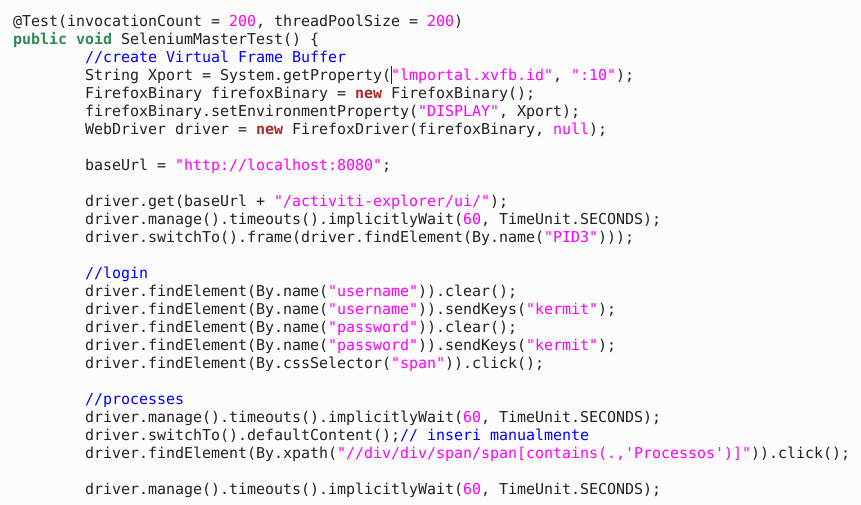
\includegraphics[width=0.9\textwidth]{figuras/codigoCargaSelenium.png}
\caption{Selenium Load Test Source Code}
\label{fig:codigoCargaSelenium}
\end{figure}


%Para a execuçao dos testes, o codigo capturado pelo Selenium foi reaproveitado do teste funcional e apenas foi necessario inserir a anotaçao do TestNG e o codigo referente ao Virtual Frame Buffer. Uma parte do codigo relativo a execuçao do teste de carga na primeira tarefa do processo simulando 200 usuarios virtuais pode ser visto na Figura X.
For the tests, the code captured by Selenium functional test was reused and it was only necessary to insert the annotation of TestNG and the code of the Virtual Frame Buffer. A part of the load test code simulating 200 virtual users in the first task of the process can be seen in Figure \ref{fig:codigoCargaSelenium}. It was possible to run the load test using the code obtained in Selenium combined with TestNG. With this test, we were able to analyze the performance of two versions of the both BPMS tools. In Table \ref{tab:foiPossivelCarga} may have seen an overview about which load tests could be performed. 

\begin{table}
\centering
%{\scriptsize
\begin{tabular}{p{3cm}|p{3cm}|p{3cm}}
\hline
BPMS and version & Load Test with JMeter & Load Test with Selenium and TestNG \\\hline
Bonita 5.7.2 & Able to run the test & Able to run the test \\\hline
Bonita 7.1.2 & Unable to run the test & Able to run the test \\\hline
Activiti 5.14 & Unable to run the test & Able to run the test \\\hline
Activiti 5.19 & Unable to run the test & Able to run the test \\\hline
\end{tabular}
%}
\caption{Overview of the load tests}
\label{tab:foiPossivelCarga}
\end{table}

\subsubsection{Load Test Results}

Due to problems reported in the previous section, load tests with JMeter could only be achieved in the implementation created with the version 5.7.2 of Bonita. In order to test the system behavior with different load levels, tests were performed with 1, 50, 100 and 200 virtual users and were analyzed requests regarding the essential steps to begin the process: Login, view the Bonita's homepage, select the process, show the first form and send the completed form. %The application is hosted on a SGI Altix XE 210 server with 24GB of RAM, accessible by a Fast Ethernet network.

The response times of each stage, depending on the number of users, can be seen in Table \ref{tab:resultadoCarga}. The most alarming results are for 200 virtual users, where the average response time on the login request was for 6.930 ms, or approximately 6 seconds, which is a high response time. The average response time for all requests in the test with 200 virtual users was 2.903 ms (i.e., 3 s). Besides high response times, the test showed virtual users 200 with error rates in some requests which were not found with a smaller number of users. For example, a request that has performed login showed a error rate of 1.99\% and, in total, the requests have obtained an error rate of 6.98\%. The errors occurred because of unanswered requests.

%\begin{table}
%{\scriptsize
%\centering
%\begin{tabular}{p{2cm}|p{2cm}|p{2cm}|p{2cm}|p{2cm}|p{2cm}}
%\hline
%Users & Login & Home Page & Process selection & First form & Send form \\\hline
%1 & 126 & 32 & 38 & 80 & 73\\\hline
%50 & 597 & 191 & 179 & 368 & 152\\\hline
%100 & 1972 & 571 & 552 & 760 & 694\\\hline
%200 & 10.149 & 3.239 & 934 & 2.122 & 1.918\\\hline
%\end{tabular}
%}
%\caption{Average response times, in milliseconds}
%\label{tab:resultadoCarga}
%\end{table}

\begin{table}
{\scriptsize
\centering
\begin{tabular}{p{2cm}|p{2cm}|p{2cm}|p{2cm}|p{2cm}|p{2cm}}
\hline
Users & Login & Home Page & Process selection & First form & Send form\\\hline
1 & 65 & 20 & 19 & 52 & 42\\\hline
50 & 387 & 101 & 92 & 260 & 90\\\hline
100 & 1072 & 490 & 473 & 601 & 564\\\hline
200 & 6.930 & 2.345 & 876 & 1.611 & 1.087\\\hline
\end{tabular}
}
\caption{Average response times, in milliseconds}
\label{tab:resultadoCarga}
\end{table}


%De forma geral, portanto, o teste de carga com JMeter atingiu seus objetivos e ajuda a explicar a sobrecarga que ocorreu com a aplicação em produção, quando muitos alunos tentaram acessar o formulário inicial numa data limite. No entanto, é importante ressaltar que este teste foi executado apenas em etapas iniciais do processo e, mesmo assim, já foi trabalhoso e consumiu algumas horas de preparação, por exigir uma análise profunda das requisições HTTP para executar os testes com sucesso. Ao todo, foram capturadas cerca de 100 requisições só nestas etapas, portanto estima-se que o teste de uma tarefa mais ao final do processo possa se tornar inviável com JMeter, por demandar a identificação e interpretação de muitas requisições. Outra observação importante, nesta experiência, é que esta abordagem de teste sofre com a dependência das tecnologias Web empregadas pelo BPMS. %pois, das quatro versoes testadas, em apenas uma delas foi possivel realizar o teste com sucesso e isso ocorreu principalmente devido a forma como os BPMS sao implementados

Overall, the load testing with JMeter helps explain the overload that occurred with the application in production, when many students tried to access the initial form in a deadline, mainly because the test with 200 users has created a charge that led some pages to stop responding. However, it is important to note that this test was performed only in the early stages of the process and, even then, was already laborious and consumed a few hours of preparation, because it requires a deep analysis of HTTP requests to run the tests successfully. In all, about 100 requests were captured only in these steps, therefore it is estimated that the testing of a task towards the end of the process can become unwieldy with JMeter, it demands the identification and interpretation of many requests. Another important observation in this experiment is that this testing approach suffers from dependence on Web technologies used by BPMS, therefore, the four versions tested in only one of them it was possible to conduct the test successfully and this was mainly due to how the BPMS are implemented.

%teste de carga com selenium + testng
On the other hand, in the load test performed with Selenium and TestNG all versions of the tools could be successfully tested. These tests were also performed simulating 1, 50, 100 and 200 virtual users/threads but, because it is a load test conducted in a different way of JMeter (without HTTP requests) could not be analyzed on isolated results of each request or the response time. At the end of the test run, the TestNG generate reports that display the time that each execution (each thread) took to complete and total test execution time. 

In the execution time is included the time of the entire interaction with the application, since this is effectively executed by each thread, different from test with JMeter where the requests are simulated and the response time is measured. For example, the average execution time of each thread in all of the tools tested and for any amount of threads was the same: about 14s. Thus, it is impossible to compare the runtime with the response time obtained in JMeter because it reflects more about client behavior than server.

However, it was possible to analyze the server behavior front a large number of simultaneous accesses from other types of information. In tests with 200 threads, for example, some threads have failed due to pages that have stopped responding, the only test that returns no errors in this case was the test with the Activiti tool in version 19.5. The server logs were also observed some errors in the lack of response. This behavior is similar to what happened with testing with JMeter. In the Table \ref{tab:resultadoCargaSelenium} can be seen in the summary of server behavior for each tool and for each number of virtual users/threads.

\begin{table}
%{\scriptsize
\centering
\begin{tabular}{p{2cm}|p{2cm}|p{2cm}|p{2cm}|p{2cm}}
\hline
Users & Bonita 5.7.2 & Bonita 7.1.2 & Activiti 5.14 & Activiti 5.19 \\\hline
1 & No failure & No failure & No failure & No failure \\\hline
50 & No failure & No failure & No failure & No failure \\\hline
100 & Some failure & No failure & No failure & No failure \\\hline
200 & Some failure & Some failure & Some failure & Some failure \\\hline
\end{tabular}
%}
\caption{Summary of server behavior}
\label{tab:resultadoCargaSelenium}
\end{table}

Thus, it can be said that the load test with TestNG achieved its objectives because it was useful to simulate a large number of users performing actions in the system simultaneously and experienced similar behavior to what was observed in tests with JMeter. The approach using TestNG and Selenium has the advantage of being possible to carry out tests on all the tools analyzed, showing that it is not dependent on the tool structure. However, as observed in other tests, the task of running the tests can become cumbersome if you need to test many tasks or many process flows. This approach also has the advantage of being able to reuse code created in the functional test, which allows shorten test creation.


\section{Considerações Finais}\label{s:conclu}
%revisar aqui
%conclusao, esperar resultados do jmeter
%Neste trabalho, explorou-se soluções de teste automatizado em uma aplicação de BPMS. Na ausência de suporte a testes de carga e funcionais nos BPMS Bonita e Activiti, aplicou-se ferramentas de teste voltadas a aplicações Web em geral. 

In this paper we explored automated test solutions at an application of BPMS. In the absence of supporting the functional and load tests in Bonita BPMS and Activiti was applied test tools intended to Web applications in general.

%No teste funcional, com a abordagem adotada, obteve-se maior sucesso na execução dos testes e observou-se uma menor dependência dos BPMS, em comparação com o teste anterior. A tarefa de teste pode vir a ser trabalhosa, principalmente quando deseja-se testar muitas tarefas e fluxos que um processo de negócio pode ter.
In the Functional test, with the approach taken, it obtained greater success in the execution of tests and low dependence was observed in relation to the BPMS because only a few page structures must be observed (names, iframes, etc). Two initial tasks of the process  were tested and some changes were necessary for the test run. Thus, because the necessary changes, the creation of functional testing can become very cumbersome, especially when you want to test many tasks and flows that a business process can have.

Regarding the load test with JMeter, it was useful to explain failures observed in previous work with the application created with Bonita 5.7.2. Also proved to be a laborious test, or even impossible, depending on the BPMS used. Experience with two different versions of two BPMS strengthened this conclusion because there were different situations, with Bonita in version 5.7.2 the test was successful, but with the others tools the test could not be executed, since it failed to reproduce all requests. On the other hand, the load test performed with Selenium and TestNG enabled all analyzed tools to be tested, making it a good alternative for load test.
%Os valores obtidos.. compara com o jmeter

%De modo geral, a experiência mostrou que, sob certas condições, é viável testar aplicações de BPMS com ferramentas de teste para sistemas Web. A principal condição, no caso considerado, foi o direcionamento dos testes a uma tarefa inicial do processo, identificada como gargalo. Como o tempo e esforço para uma única tarefa foi significativo, essa abordagem pode se tornar inviável caso seja necessário aumentar a cobertura dos testes.

%De modo geral, como lições aprendidas temos que, sob certas condições, é viável testar aplicações de BPMS com ferramentas de teste para sistemas Web. A principal condição, no caso considerado, foi o direcionamento dos testes a uma tarefa inicial do processo, identificada como gargalo. Como o tempo e esforço para uma única tarefa foi significativo, essa abordagem pode se tornar inviável caso seja necessário estender os testes a muitas tarefas de um processo.
Overall, how lessons learned we have that under certain conditions it is feasible to test application of BPMS with testing tools for Web systems. The main condition in the case considered, was the targeting of testing an initial task of the process, identified as neck. As the time and effort to a single task was significant, this approach can become unwieldy if necessary extend the tests to many tasks of a process.

Another aspect to consider is that when the BPMS implements the interaction with the user and/or servers, the developer do not to choose and control all technologies used. This facility, however, may make it difficult to test automation with external tools, that benefit from knowledge about the implementation (eg, use of \emph{iframes}, Ajax, in the experience in question).

%Embora a experiência deste trabalho não tenha sido exaustiva, pôde-se notar que o suporte a testes automatizados é pouco explorado em BPMS. Entende-se que esta seria uma funcionalidade bem-vinda, supondo-se que abreviaria uma etapa essencial para garantir a qualidade do software resultante. 

Although the experience of this work was not exhaustive, it might be noted that support automated testing is underexplored in BPMS. It is understood that this would be a welcome feature, assuming that shorten an essential step to ensure the quality of the resulting software.

\begin{thebibliography}{4}

\bibitem{weske}
Weske, M.: Business Process Management: Concepts, Languages, Architectures. Springer, 2nd edition, (2012)

\bibitem{aalst2013survey}
van~der Aalst, W. M.~P.: Business process management: A comprehensive survey. {\em ISRN Software Engineering}, 2013(507984)

\bibitem{graham2012experiences}
Graham, D. and Fewster, M.: Experiences of Test Automation: Case Studies of Software Test Automation. Addison-Wesley (2012)

\bibitem{sbsi2013}
de~Moura, J.~L. et~al.: Gestão de processos de negócio em curso de sistemas de
  informação: Relato de experiência utilizando software livre. In {\em IX Simpósio Brasileiro de Sistemas de Informação}, pp.
  206--217, (2013)

\bibitem{ABPMP} Guide to the Business Process Management Body of Knowledge (BPM
  CBOK). Association of Business Process Management Professionals, 2nd
  edition (2012)

\bibitem{forrester}
Forrester Research.: The forrester wave: {BPM} suites, {Q1} (2013)
Graham, D. and Fewster, M.

\bibitem{sbqs2015}
de Moura, J.L. and Charão, A.: Automação de Testes em Aplicações de BPMS: um Relato de Experiência. In {\em XIV Simpósio Brasileiro de Qualidade de Software}, pp.
  212--219, (2015)

\bibitem{greenresearch}
Winter Green Research.: Business process management (BPM) cloud, mobile, and patterns: Market shares, strategies, and forecasts, worldwide, 2013 to 2019.

\bibitem{swebok14}
Bourque, P. e Fairley, R.~E.: Guide to the Software Engineering Body of Knowledge (SWEBOK), Version 3.0. IEEE Computer Society (2014)

\bibitem{evoke} Chetty, N.~K.: How to perform workflow testing for BPM applications (2014), \url{http://www.evoketechnologies.com}

%\bibitem{sbqs2013}
%Chiavegatto, R. et~al.: Especificação e automação colaborativas de testes utilizando a técnica {BDD}. In {\em XII Simpósio Brasileiro de Qualidade de Software}, pp.
 % 334--341, (2013)

\bibitem{bindal2014test}
Bindal, P. and Gupta, S.: Test Automation Selenium WebDriver using TestNG. In {\em Journal of Engineering Computers \& Applied Sciences}, pp.
  18--40, (2014)

%\bibitem{myers}
%Myers, G.~J. and Sandler, C.: The Art of Software Testing. John Wiley \& Sons, (2011)


\end{thebibliography}


\end{document}

